\section{Směrová derivace, tečná rovina a normála, Taylorův polynom}
\begin{enumerate}

\item Vektor parciálních derivací nazveme gradient funkce
$$
\vec{\grad}f = (f^\prime_x; f^\prime_y)
$$
Geometrický význam gradientu: gradient je směr největšího růstu funkce.

%\item Geometrický význam gradientu: gradient je směr největšího růstu funkce.
%\item Vypočtěte gradient následujících funkcí v daných bodech:

\item Mějme $f:\mathbb{R}^2 \to \mathbb{R}$ reálnou funkci dvou reálných proměnných, bod $X = [x_0;y_0] \in D(f)$ a jednotkový vektor $\vec{s} = (s_x;s_y), |\vec{s}|=1$.

Bodem $[x_0;y_0]$ veďme rovinu $\sigma$ ve směru vektoru $\vec{s}$ kolmou na rovinu $xy$, průnik této roviny s grafem funkce $f(x,y)$ označme jako funkci $f_s$. Tečnu k této funkci v bodě $f_s(x_0;y_0)$ označme $t$. Směrnice tečny $t$ vzhledem k rovině $xy$ se nazývá směrová derivace.

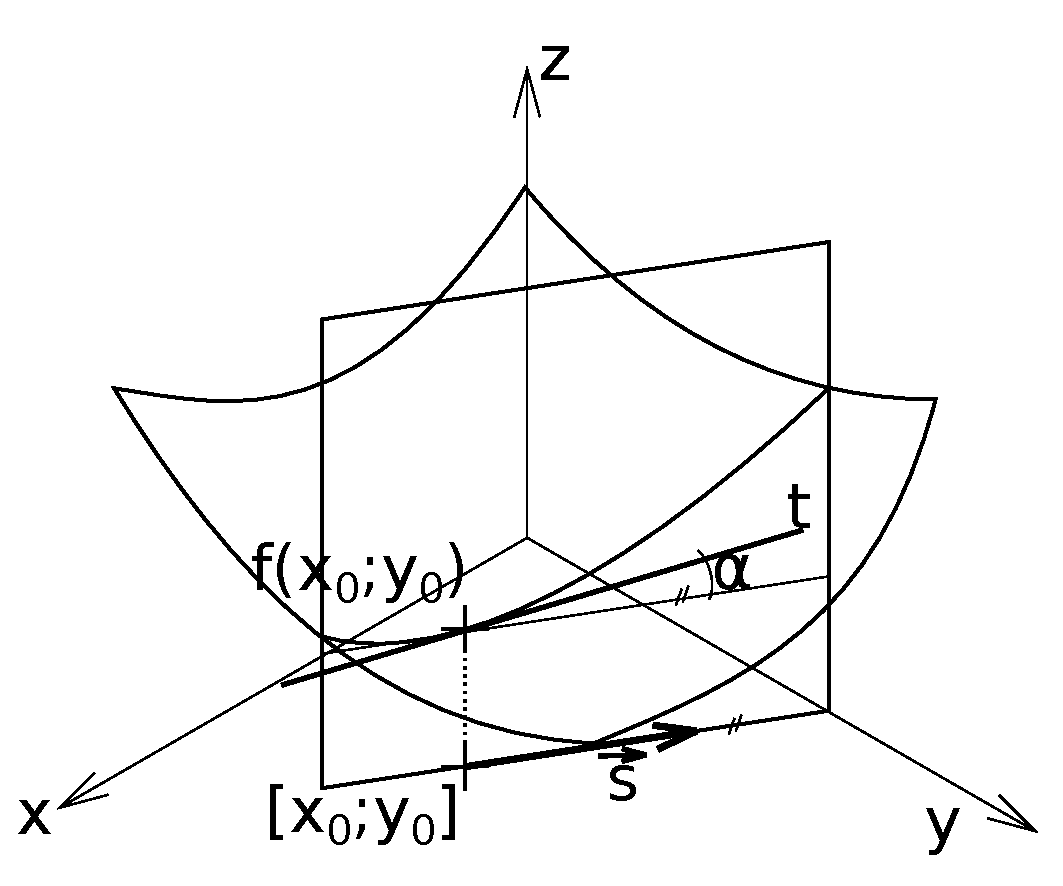
\includegraphics[scale=0.5]{Obrazky/SmerDer.pdf}

\item Směrovou derivaci lze vypočítat pomocí parciálních derivací funkce jako skalární součin směrového vektoru $\vec{s}$ s gradientem funkce $\vec{\grad}f$. 
$$
f^\prime_s = \vec{\grad} f \cdot \vec{s} 
           = (f^\prime_x; f^\prime_y) \cdot (s_x;s_y)
           = f^\prime_x \cdot s_x + f^\prime_y \cdot s_y
$$

\item Vypočtěte směrovou derivaci funkce $u(x;y)$ ve směru vektoru $\vec{s}$:
\begin{enumerate}
\item[a)]{$u=x^4+y^4-4x^2y^2$}, $\vec{s}=(1;1)$
\hspace{\fill}[$2\sqrt{2}[(x^3+y^3) - 2(x+y)]$]
\item[b)]{$u=xy+\frac{x}{y}$}, $\vec{s}=(1;-1)$
\hspace{\fill}[$\frac{\sqrt{2}}{2} (y-x+\frac{1}{y}+\frac{x}{y^2})$]
\item[c)]{$u=\frac{x}{y^2}$}, $\vec{s}=(2;1)$
\hspace{\fill}[$\frac{2\sqrt{5}}{5y^2}(1+\frac{x}{y})$]
\end{enumerate}

\item Vypočtěte směrovou derivaci funkce $u(x;y)$ ve směru vektoru $\vec{s}$ v bodě $[x_0;y_0]$:
\begin{enumerate}
\item[a)]{$u=x\sin(x+y)$}, $\vec{s}=(4;-3)$, $[x_0;y_0]=[\pi;\pi]$
\hspace{\fill}[$\frac{\pi}{5}$]
\item[b)]{$u=\ln(x+y^2)$}, $\vec{s}=(3;-4)$, $[x_0;y_0]=[2;1]$
\hspace{\fill}[$-\frac{1}{3}$]
\item[c)]{$u=(x^2y+y)^4$}, $\vec{s}=(5;12)$, $[x_0;y_0]=[2;-3]$
\hspace{\fill}[$0$]
\end{enumerate}

\item Najděte tečnou rovinu a normálu funkce $f(x;y)$ v bodě $A[x_0;y_0]$:
\begin{enumerate}
\item[a)]{$u=x^4+y^4-4x^2y^2$}, $A[3;2]$
\hspace{\fill}[$\vec{n}=(-12;112;1)$]
\item[b)]{$u=x\sin(x+y)+5$}, $A[\pi;\pi]$
\hspace{\fill}[$\vec{n}=(-\pi,-\pi,1)$]
\end{enumerate}

\item Taylorovým polynomem řádu $r$ se středem v bodě $A$ se rozumí polynom:
$$
t_{A,r} = \sum_{i=0}^r \frac{\mathrm{d}^i f_A}{i!}
\mathrm{, ~ kde ~ }
\mathrm{d}^r f_A = \left( \sum_{i=1}^m \frac{\partial}{\partial x_i} \mathrm{d}x_i \right)^r (f(A))
$$
je tzv. $r$-tý diferenciál. Kupř. (pro fci dvou proměnných):
\\$\mathrm{d}^0 f_A = f(A)$
\\$\mathrm{d}^1 f_A = \mathrm{d} f(A)$
\\$\mathrm{d}^2 f_A = (\frac{\partial}{\partial x} \mathrm{d}x
                     + \frac{\partial}{\partial y} \mathrm{d}y)^2
                     \cdot(f(A))
                    = (\frac{\partial^2}{\partial x^2} \mathrm{d}x^2
                     +2\frac{\partial^2}{\partial x \partial y} 
                       \mathrm{d}x \mathrm{d}y
                     + \frac{\partial^2}{\partial y^2} \mathrm{d}y^2)
                     \cdot(f(A))
                     $
\\$                 = \frac{\partial^2 f}{\partial x^2} (A) \mathrm{d}x^2
                    +2\frac{\partial^2 f}{\partial x \partial y} (A)
                        \mathrm{d}x \mathrm{d}y
                    + \frac{\partial^2 f}{\partial y^2} (A) \mathrm{d}y^2
                     $
\\$\mathrm{d}^3 f_A = \frac{\partial^3 f}{\partial x^3} (A) \mathrm{d}x^3
                    +3\frac{\partial^3 f}{\partial x^2 \partial y} (A)
                        \mathrm{d}x^2  \mathrm{d}y
                    +3\frac{\partial^3 f}{\partial x \partial y^2} (A)
                        \mathrm{d}x \mathrm{d}y^2     
                    + \frac{\partial^3 f}{\partial y^3} (A) \mathrm{d}y^3
                     $
                     
                     
\item Určete diferenciál funkce $f$ v bodě $A$
\begin{enumerate}
    \item[a)] $f=e^x\cos{y},A=[0,0]$ \hspace{\fill} [$\mathrm{d}x$] 
    \item[b)] $f=\frac{1}{x^2+y^2},A=[-1,2]$ \hspace{\fill} [$\frac{2}{25}\mathrm{d}x-\frac{4}{25}\mathrm{d}y$]
    \item[c)] $f=\frac{x^2-y^2}{xy},A=[2,2]$, při přírůstku $\vec{h}=(0.03,0.01)$ \hspace{\fill} [$0.02$]
\end{enumerate}

\item Určete druhý diferenciál funkce $f$ v bodě $A$
\begin{enumerate}
    \item[a)] $f=e^{xy},A=[0,0]$ \hspace{\fill} [$2\mathrm{d}x\mathrm{d}y$]
    \item[b)] $f=x^2y^2,A=[1,1]$ \hspace{\fill} [$2\mathrm{d}x^2+8\mathrm{d}x\mathrm{d}y+2\mathrm{d}y^2$]
\end{enumerate}
                     
\item Určete Taylorův polynom příslušného stupně $n$ dané funkce $f(x;y)$ se středem v bodě $A=[x_0;y_0]$
\begin{enumerate}
\item[a)]{$f(x;y)=\ln(\sqrt{x^2+y^2})$}, $n=2$, $A=[-1;-1]$
\hspace{\fill}[$\frac{1}{2}(\ln(2) -xy-2x-2y-3)$]
\item[b)]{$f(x;y)=\sin(x+y)$}, $n=3$, $A=[\frac{\pi}{2};\frac{\pi}{2}]$
\hspace{\fill}[$-x-y+\pi+\frac{1}{3}(\ldots)$]
\item[c)]{$f(x;y)=2x^2-xy-y^2-6x-3y+5$}, $n=3$, $A=[1;-2]$
\end{enumerate}

                     
\item Určete Maclaurinov polynom příslušného stupně $k$ dané funkce $f(x;y)$
\begin{enumerate}
\item[a)]{$f(x;y)=(1+x)^m(1+y)^n$}, $n,m \in \mathbb{N}$, $k \in \mathbb{N}$
\hspace{\fill}[$1+mx+ny+\frac{m(m-1)}{2!}x^2+mnxy+\frac{n(n-1)}{2!}y^2+...$]
\item[b)]{$f(x;y)=\ln(1+x+y)$}, $k=3$
\hspace{\fill}[$x+y-\frac{x^2}{2}-xy-\frac{y^2}{2}+\frac{x^3}{3}+x^2y+xy^2+\frac{y^3}{3}$]
\item[c)]{$f(x;y)=e^x\sin(y)$}, $k=3$
\hspace{\fill}[$y+xy+\frac{1}{3!}(3x^2y-y^3)$]
\item[d)]{$f(x;y)=e^x\cos(y)$}, $k=3$
\hspace{\fill}[$1+x+\frac{1}{2}(x^2-y^2)+\frac{1}{3!}(x^3-3xy^2)$]
\item[e)]{$f(x;y)=\sin(x^2+y^2)$}, $k=3$
\hspace{\fill}[$x^2+y^2$]
\item[f)]{$f(x;y)=\ln(1+x)\ln(1+y)$}, $k=3$
\hspace{\fill}[$xy-\frac{1}{2}(x^2y+xy^2)$]
\end{enumerate}
\end{enumerate}